%!TEX root = ../document.tex

\section{Example Section}
\label{sect:example-section}

\sideboxbegin{o}
\spar
\sideboxend

\stext[2-7]

\subsection{Example Image}

\stext[7-10]

\begin{figure}
  \centering
  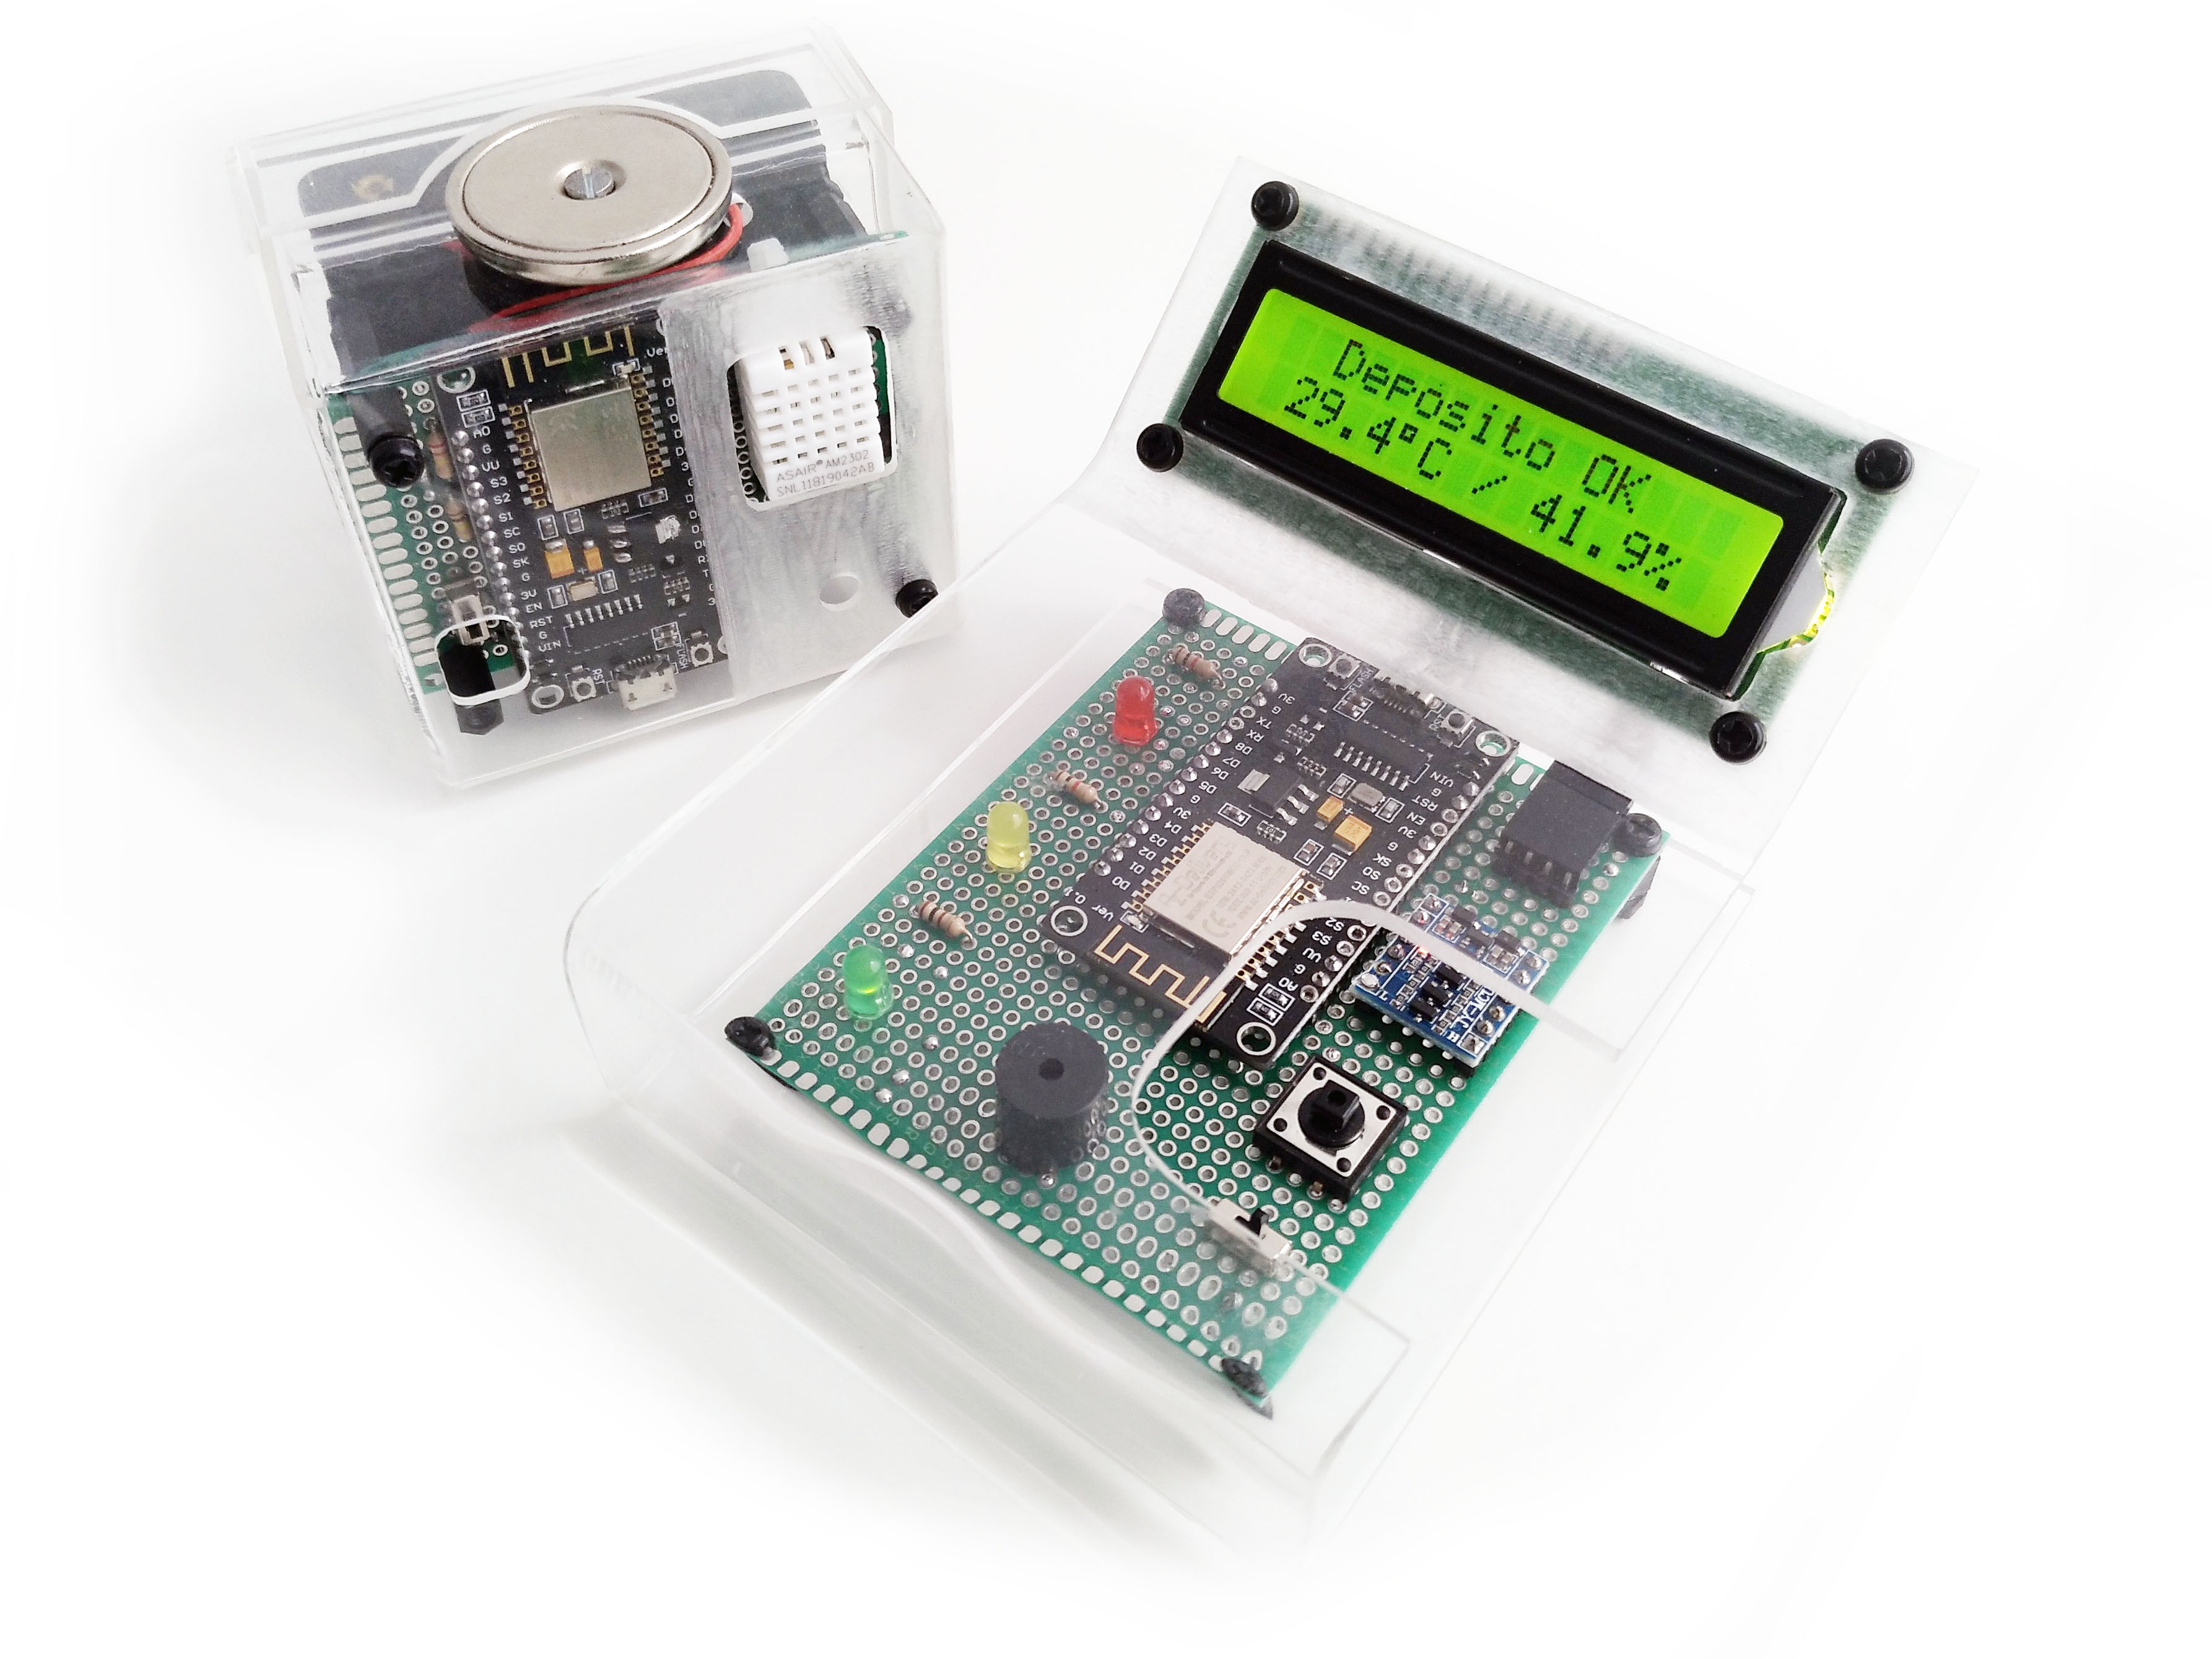
\includegraphics[width=1\columnwidth]{../photos/chanams-front}
  \caption{Example Figure}
  \label{fig:example}
\end{figure}

\subsection{Example Tables}

%!TEX root = ../document.tex

\begin{table}
\caption{Example table}
\label{tab:example}
\begin{tabularx}{\textwidth}{ccX}
\toprule
\headingc{Col. 1} & \headingc{Col. 2} & \headingc{Col. 3} \\
\topruleb
A
&
Row 1
&
Nunc sed pede. Praesent vitae lectus. Praesent neque justo, vehicula eget, interdum id, facilisis et, nibh. Phasellus at purus et libero lacinia dictum. Fusce aliquet. Nulla eu ante placerat leo semper dictum. Mauris metus. Curabitur lobortis. Curabitur sollicitudin hendrerit nunc. Donec ultrices lacus id ipsum.
\\*\midrule
B
&
Row 2
&
Nunc sed pede. Praesent vitae lectus. Praesent neque justo, vehicula eget, interdum id, facilisis et, nibh. Phasellus at purus et libero lacinia dictum. Fusce aliquet. Nulla eu ante placerat leo semper dictum. Mauris metus. Curabitur lobortis. Curabitur sollicitudin hendrerit nunc. Donec ultrices lacus id ipsum.
\\*\midrule
C
&
Row 3
&
Nunc sed pede. Praesent vitae lectus. Praesent neque justo, vehicula eget, interdum id, facilisis et, nibh. Phasellus at purus et libero lacinia dictum. Fusce aliquet. Nulla eu ante placerat leo semper dictum. Mauris metus. Curabitur lobortis. Curabitur sollicitudin hendrerit nunc. Donec ultrices lacus id ipsum.
\\*\midrule
D
&
Row 4
&
Nunc sed pede. Praesent vitae lectus. Praesent neque justo, vehicula eget, interdum id, facilisis et, nibh. Phasellus at purus et libero lacinia dictum. Fusce aliquet. Nulla eu ante placerat leo semper dictum. Mauris metus. Curabitur lobortis. Curabitur sollicitudin hendrerit nunc. Donec ultrices lacus id ipsum.
\\*\bottomrule

\end{tabularx}
\end{table}

\stext[11-15]

\LTXtable{\textwidth}{tables/example-long-table}

\sspar

\subsection{Example citations}

\sspar

\begin{fancyquote}{Author}
\sspar
\end{fancyquote}

\subsection{Example boxes}

\sspar

\examplebegin{Example title}
\sspar
\exampleend

\tipbegin{Tip title}
\sspar
\tipend

\tnotebegin{Note title}
\sspar
\tnoteend

\subsection{Compact enumerations}

\sspar

\begin{itemizecompact}
  \item \sspar
  \item \sspar
\end{itemizecompact}

\sspar

\begin{enumeratecompact}
  \item \sspar
  \item \sspar
\end{enumeratecompact}

\sspar

\begin{descriptioncompact}
  \item [Item 1] --- \sspar
  \item [Item 2] --- \sspar
\end{descriptioncompact}

\subsection{Example listings}

\sspar

\begin{lstlisting}[
language=bash,
caption=Hello world! 
]
#!/bin/bash
STR="Hello World!"
echo $STR
\end{lstlisting}

\sspar

\begin{lstlisting}[
language=bash,
caption=Hello World! in QVT-o,
style=QVT
]
modeltype ABC uses ABC('http:///ABC.ecore');

transformation HelloWorld(in source:ABC, out target:ABC);

main() {
  source.rootObjects()[Root]->map Root2Root();
}

mapping Root :: Root2Root() : Root {
  element += self.element->select(a |
    a.oclIsKindOf(A))[A]->map A2B();
}

mapping A :: A2B() : B
  when {
    self.id > 0
  }
  {
  result.id := self.id;
  result.b := self.a + " World!";
}
\end{lstlisting}

\subsection{Example UML diagrams}

\sspar

\begin{figure}
\centering

\begin{tikzpicture}[node distance=2em and 2em]
\node (A) [
  class
] at (0, 0) {
  \stereotype{stereotype1}
  A
  \attributes{
    name : String [1]\\
    size : Integer [0..1]
  }
};

\node (B) [
  classop,
  right = 4cm of A
] {
  B
  \attributes{
    \ldots
  }
  \operations{
    do()
  }
};

\node (C) [
  class
] at ($(A)!0.5!(B) + (0, -2)$) { % Between A and B, 2 units below
  C
};

\draw [contains] (A) -- (B);
\draw [assoc] (A) |- (C);
\end{tikzpicture}
\caption{Example class diagram}
\end{figure}

\begin{figure}
\centering
\begin{tikzpicture}[node distance=2em and 2em]
\node (a) [
  object,
] {
  \obj{a}{A}
  \attributes{
    name : 'a'\\
    size : 10
  }
};

\node (B) [
  object,
  right = of a
] {
  \obj{b}{B}
};

\end{tikzpicture}
\caption{Example object diagram}
\end{figure}

\sspar
